\documentclass[a4paper, 12pt]{article}
\usepackage[utf8x]{inputenc}
\usepackage{cmap}
\usepackage[english, russian]{babel}
\usepackage{indentfirst}
\usepackage[left=20mm, top=20mm, right=20mm, bottom=20mm]{geometry}
\usepackage{tikz}
\usepackage{float}
\usepackage{amsmath, amsfonts, amssymb}
\usepackage{graphicx}
\usepackage{fancybox, fancyhdr}
\usepackage{hyperref}
\usepackage{listings}
\usepackage{caption}
\usepackage{subcaption}
\usepackage{xcolor}
\pagestyle{fancy}
\fancyhf{}
\fancyhead[L]{Лабораторная работа №1}
\fancyhead[R]{Математическая статистика}
\fancyfoot[C]{\thepage}
\graphicspath{{images/}}
\usetikzlibrary{patterns}
\definecolor{LightGray}{gray}{0.95}
\definecolor{LightGray2}{gray}{0.7}
\lstdefinestyle{code}{
    language=Python, % replace with needed language
    basicstyle=\footnotesize\ttfamily,
    % numbers=left,
    % numberstyle=\scriptsize\color{gray},
    % stepnumber=1,
    % numbersep=5pt,
    backgroundcolor=\color{LightGray},
    showspaces=false,
    showstringspaces=false,
    showtabs=false,
    tabsize=4,
    captionpos=b,
    breaklines=true,
    breakatwhitespace=false,
    frame=single,
    rulecolor=\color{LightGray2},
    linewidth=\linewidth,
    keywordstyle=\color{blue}\bfseries,
    commentstyle=\color{green!40!black},
    stringstyle=\color{purple},
    escapeinside={\%*}{*)},
    inputencoding=utf8x,
    xleftmargin=0pt,
    framexleftmargin=0pt,
    framexrightmargin=0pt
}
\lstset{style=code}
\hypersetup{
    colorlinks=true,
    linkcolor=blue,
    filecolor=magenta,
    urlcolor=cyan,
    pdftitle={contents setup},
    pdfpagemode=FullScreen,
}
\setlength{\parskip}{1.5mm}
\setlength{\headheight}{15pt}
\setlength{\footskip}{15pt}
\allowdisplaybreaks
\DeclareMathOperator{\sinc}{sinc}
\newcommand{\frc}[2]{\raisebox{2pt}{$#1$}\big/\raisebox{-3pt}{$#2$}}

\begin{document}
    \begin{titlepage}

        \begin{center}
        
\includegraphics[width=0.3\textwidth]{itmo.png} % requires itmo.png in /images folder
        \vfill
        
        Федеральное государственное автономное образовательное учреждение высшего образования
        «Национальный Исследовательский Университет ИТМО»\\
        
        \vfill
        {\large\bf ЛАБОРАТОРНАЯ РАБОТА №1}\\
        {\large\bf ПРЕДМЕТ «МАТЕМАТИЧЕСКАЯ СТАТИСТИКА»}\\
        Вариант 4, 2
        \vfill

        \begin{flushright}
            \begin{minipage}{.45\textwidth}
            {
                \hbox{Преподаватель: Лимар И. А.}
                \hbox{Студент: Румянцев А. А.}
                \hbox{Поток: Мат Стат 31.2}
                \hbox{}
                \hbox{Факультет: СУиР}
                \hbox{Группа: R3341}
            }
            \end{minipage}
        \end{flushright}
        
        \vfill
                
        Санкт-Петербург\\
        2024
        \end{center}
    \end{titlepage}
    
    \tableofcontents

    \newpage
    \section{Задание 1}
    \subsection{Условие}
    В файле mobile\_{phones}.csv приведены данные о мобильных телефонах. В сколько моделей
    можно вставить 2 сим-карты, сколько поддерживают 3-G, каково наибольшее число ядер
    у процессора? Рассчитайте выборочное среднее, выборочную дисперсию, выборочную медиану
    и выборочную квантиль порядка 2/5, построить график эмпирической функции
    распределения, гистограмму и box-plot для емкости аккумулятора для всей совокупности
    и в отдельности для поддерживающих/не поддерживающих Wi-Fi


    \subsection{Выполнение}
    Для начала импортируем необходимые библиотеки
    \begin{lstlisting}[label=import, caption={Импортирование библиотек}]
    import numpy as np
    import pandas as pd
    import matplotlib.pyplot as plt
    \end{lstlisting}


    Теперь считаем таблицу по ссылке на представленный гугл-диск в переменную df
    \begin{lstlisting}[label=read, caption={Считывание таблицы}]
    url='https://drive.google.com/file/d/1O4rFr9xg9aFmkjx4-hl_XOc5O9q65_EW\
        /view?usp=sharing'
    url='https://drive.google.com/uc?id=' + url.split('/')[-2]
    df = pd.read_csv(url)
    \end{lstlisting}


    В колонках <<dual\_{sim}>> и <<three\_{g}>> наличие или отсутствие параметра определяется
    единицей или нулем соответственно, следовательно, просуммировав значения в этих столбцах,
    получим количество моделей с наличием данных параметров. Для ядер просто выведем максимум
    из столбца. Используем методы библиотеки \texttt{pandas} -- \texttt{sum} и \texttt{max}
    \begin{lstlisting}[label=3q, caption={Код на ответы на первые три вопроса}]
    # how many models can you insert 2 SIM cards into?
    dual_sim_count = df['dual_sim'].sum()
    print(f'dual_sim_count={dual_sim_count}')
        
    # how many models support 3-G?
    three_g_count = df['three_g'].sum()
    print(f'three_g_count={three_g_count}')
        
    # what is the highest number of cores a processor has?
    max_cores = df['n_cores'].max()
    print(f'max_cores={max_cores}')
    \end{lstlisting}

    
    Получим следующий вывод в консоль
    \begin{lstlisting}[label=3qa, caption={Вывод в консоль: ответы на первые три вопроса}]
    dual_sim_count=1019
    three_g_count=1523
    max_cores=8
    \end{lstlisting}


    Для расчета необходимых характеристик я написал отдельный метод, куда достаточно
    передать выборку и ее именование для удобного вывода в консоль. Используем методы
    библиотеки \texttt{pandas} -- \texttt{mean} посчитает выборочное среднее,
    \texttt{var} выборочную дисперсию, \texttt{median} выборочную медиану и \texttt{quantile}
    с параметром \texttt{q=2/5} квантиль порядка 2/5
    \begin{lstlisting}[label=mvals, caption={Код для подсчета основных характеристик}]
    # calculating the main values
    def calculate_print_values(df: pd.Series, name: str):
        mean = df.mean()
        print(f'mean_{name}={mean}')
        
        var = df.var()
        print(f'var_{name}={var}')
        
        median = df.median()
        print(f'median_{name}={median}')
        
        quantile_2d5 = df.quantile(q=2/5)
        print(f'quantile_2/5_{name}={quantile_2d5}')
    \end{lstlisting}


    Зададим сразу три выборки -- всю, только модели с наличием Wi-Fi и только с отсутствием.
    Для составления выборок с конкретным значением требуемого параметра берем нужный столбец
    и составляем построчную связку индекс-булеан, где значением будет являться результат проверки заданного условия.
    Обращаемся к исходной таблице по этой связке и получаем новую таблицу только с теми строками, для которых по индексу
    значение было равным \texttt{True}, то есть условие выполнилось. Далее от полученной таблицы отбираем столбец по условию задания.
    Для удобного вывода добавим метод разделитель, который будем вызывать между операциями с выборками.
    Вызовем подсчитывающий метод три раза для трех выборок
    \begin{lstlisting}[label=mvals2, caption={Подготовка для удобного и быстрого получения результатов}]
    # common separator between unrelated outputs
    def print_separate():
        print('----------------')

    # the entire sample
    all_battery = df['battery_power']
    calculate_print_values(all_battery, name='all_battery')

    print_separate()

    # selection with the condition of wifi availability
    wifi_table = df[df['wifi']==1]
    wifi_battery = wifi_table['battery_power']
    calculate_print_values(wifi_battery, name='wifi_battery')

    print_separate()

    # selection with the condition of wifi unavailability
    nowifi_table = df[df['wifi']==0]
    no_wifi_battery = nowifi_table['battery_power']
    calculate_print_values(no_wifi_battery, name='no_wifi_battery')
    \end{lstlisting}


    С заданными ранее параметрами получаем следующий вывод в консоль
    \begin{lstlisting}[label=mvalsout, caption={Вывод в консоль: посчитанные основные характеристики}]
    mean_all_battery=1238.5185
    var_all_battery=193088.35983766883  
    median_all_battery=1226.0
    quantile_2/5_all_battery=1076.0     
    ----------------
    mean_wifi_battery=1234.9043392504932
    var_wifi_battery=190296.40051422242 
    median_wifi_battery=1233.0
    quantile_2/5_wifi_battery=1077.8000000000002
    ----------------
    mean_no_wifi_battery=1242.235294117647      
    var_no_wifi_battery=196128.43798148702      
    median_no_wifi_battery=1222.0
    quantile_2/5_no_wifi_battery=1076.0
    \end{lstlisting}


    Теперь построим графики в соответствии с заданием.
    Напишем метод, который принимает выборку и название графика -- таким образом, достаточно
    будет вызвать метод для каждой выборки и получить все графики. Используем библиотеку 
    \texttt{matplotlib} для отрисовки, \texttt{pandas} для подсчета необходимых данных.
    Для построения графика эмпирической функции распределения находим
    по сортированным данным без сохранения индексов связку ключ-значение, где ключ --
    \texttt{battery\_{power}}, значение -- вероятность встретить именно такую \texttt{battery\_{power}}.
    После составляем кумулятивные суммы по этим вероятностям. Для гистограммы определяем
    количество интервалов правилом Стёрджеса: $n=1+\log_2{N}$ и округляем вниз
    \begin{lstlisting}[label=graps, caption={Код для построения необходимых графиков}]
    # plotting basic graphs
    def show_graphs(df: pd.Series, name='sample'):
        # the resulting axis will be labeled 0, 1, ..., n - 1
        sorted_ = df.sort_values(ignore_index=True)

        # normalize for proportions (probabilities) instead of freqs
        # sorting by DataFrame column values (not by freqs)
        idx_prob = sorted_.value_counts(normalize=True, sort=False)

        # parsing x & y then cumsum for distribution function
        plt.plot(idx_prob.index, idx_prob.values.cumsum())
        plt.title(f'Empirical distribution function of {name}')
        plt.xlabel('battery_power')
        plt.ylabel('probability')
        plt.grid()
        plt.gcf().set_size_inches(10, 5)
        plt.show()

        # Sturges' rule
        n = np.int64(np.floor(1+3.322*np.log10(df.shape[0])))
        plt.hist(df, bins=n)
        plt.title(f'Histogram of {name}')
        plt.xlabel('battery_power')
        plt.ylabel('count')
        plt.grid()
        plt.gcf().set_size_inches(10, 5)
        plt.show()

        plt.boxplot(df)
        plt.title(f'Boxplot of {name}')
        plt.ylabel('battery_power')
        plt.grid()
        plt.gcf().set_size_inches(10, 5)
        plt.show()
    \end{lstlisting}


    \begin{figure}[H]
        \centering
        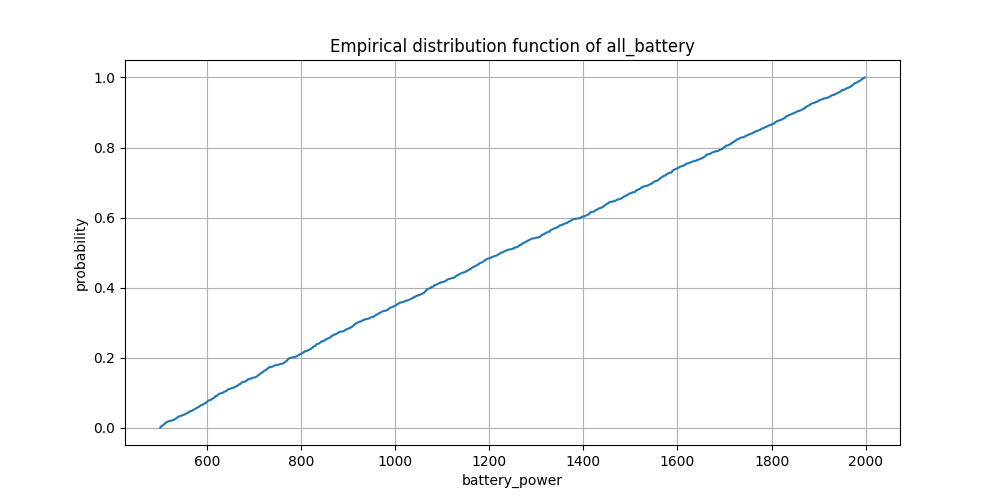
\includegraphics[scale=0.55]{all_battery_edf.png}
        \captionsetup{skip=0pt}
        \caption{График эмпирической функции распределения для всей выборки}
        \label{fig:allbedf}
    \end{figure}
    \begin{figure}[H]
        \centering
        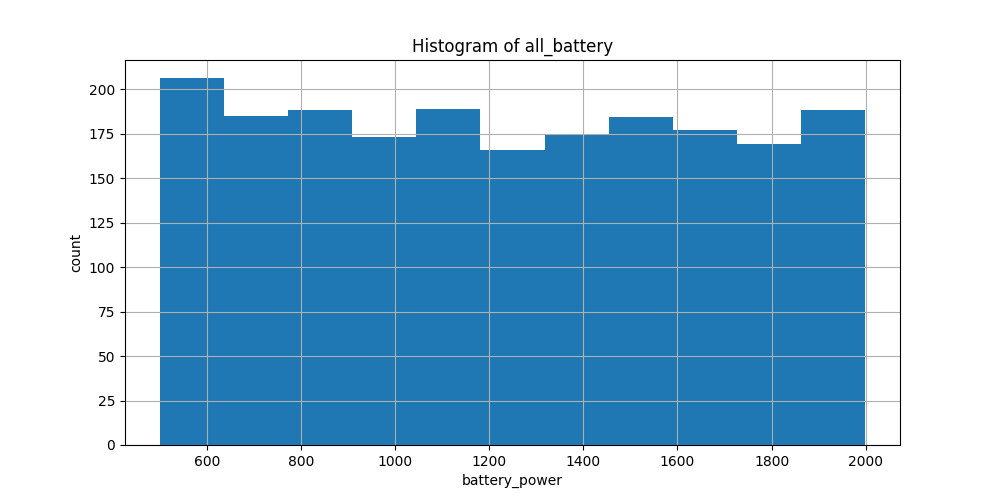
\includegraphics[scale=0.55]{all_battery_hist.png}
        \captionsetup{skip=0pt}
        \caption{Гистограмма для всей выборки}
        \label{fig:allbhist}
    \end{figure}
    \begin{figure}[H]
        \centering
        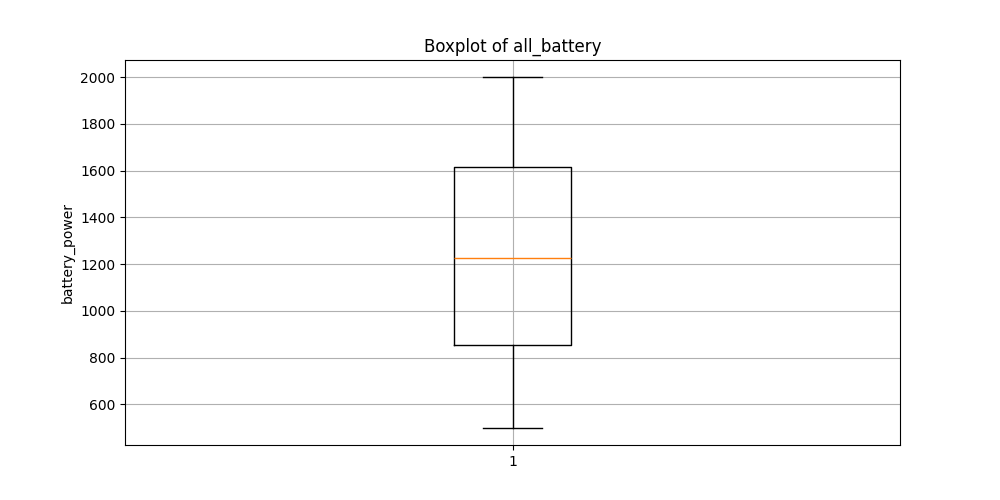
\includegraphics[scale=0.55]{all_battery_box.png}
        \captionsetup{skip=0pt}
        \caption{Ящик с усами для всей выборки}
        \label{fig:allbbox}
    \end{figure}


    \begin{figure}[H]
        \centering
        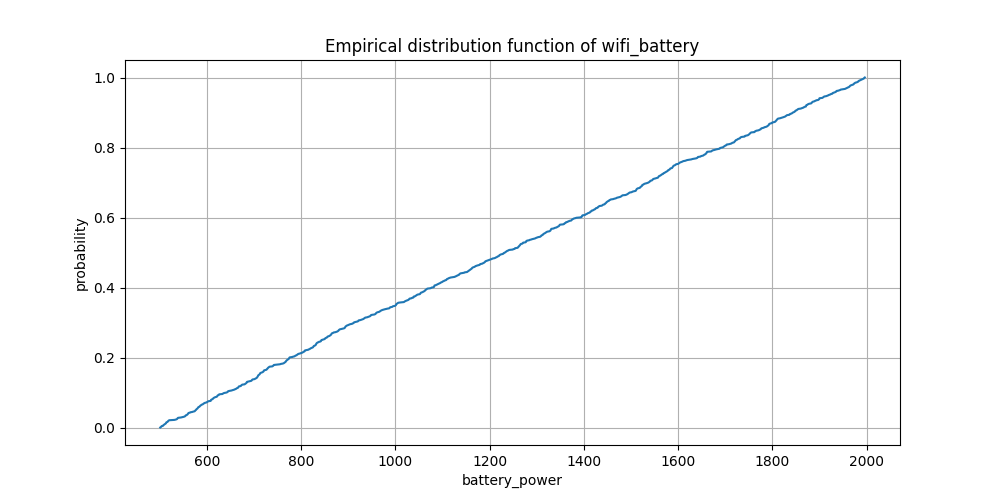
\includegraphics[scale=0.55]{wifi_battery_edf.png}
        \captionsetup{skip=0pt}
        \caption{График эмпирической функции распределения для выборки моделей с Wi-Fi}
        \label{fig:wifibedf}
    \end{figure}
    \begin{figure}[H]
        \centering
        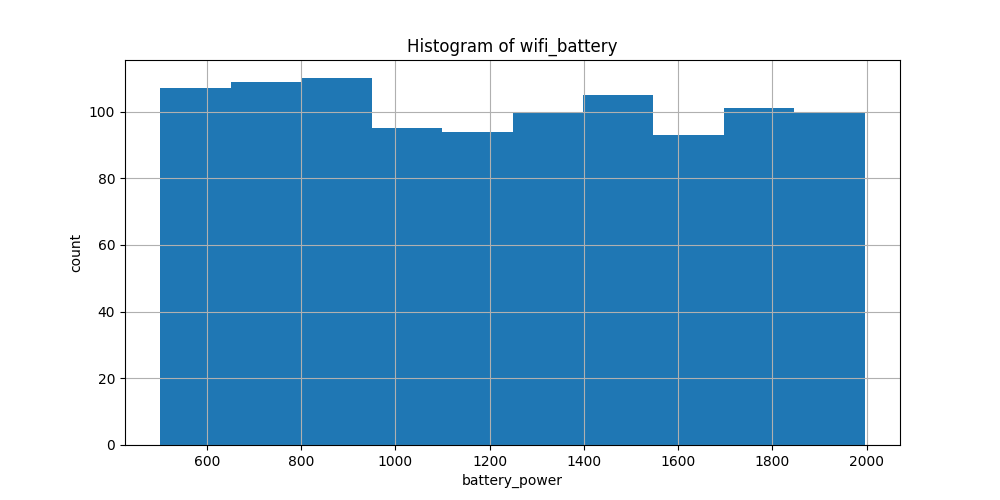
\includegraphics[scale=0.55]{wifi_battery_hist.png}
        \captionsetup{skip=0pt}
        \caption{Гистограмма для выборки моделей с Wi-Fi}
        \label{fig:wifibhist}
    \end{figure}
    \begin{figure}[H]
        \centering
        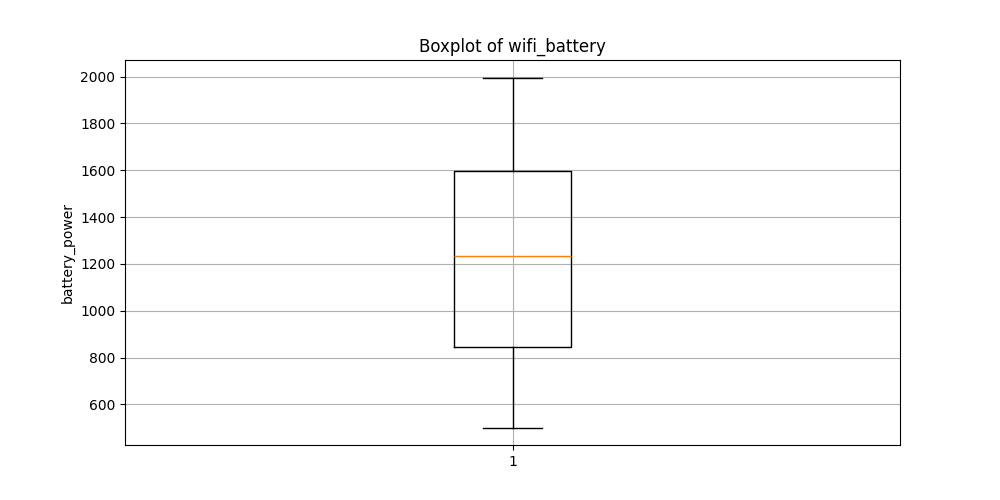
\includegraphics[scale=0.55]{wifi_battery_box.png}
        \captionsetup{skip=0pt}
        \caption{Ящик с усами для выборки моделей с Wi-Fi}
        \label{fig:wifibbox}
    \end{figure}


    \begin{figure}[H]
        \centering
        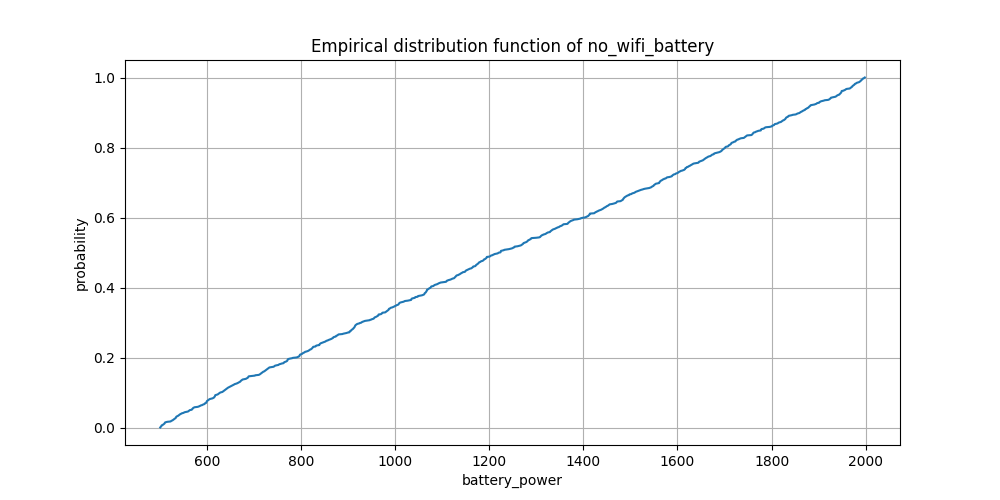
\includegraphics[scale=0.55]{no_wifi_battery_edf.png}
        \captionsetup{skip=0pt}
        \caption{График эмпирической функции распределения для выборки моделей без Wi-Fi}
        \label{fig:nowifibedf}
    \end{figure}
    \begin{figure}[H]
        \centering
        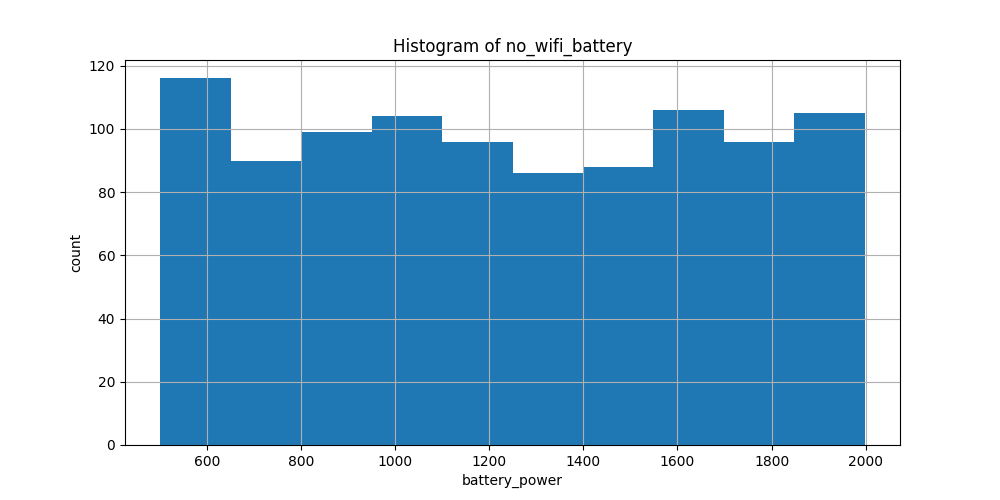
\includegraphics[scale=0.55]{no_wifi_battery_hist.png}
        \captionsetup{skip=0pt}
        \caption{Гистограмма для выборки моделей без Wi-Fi}
        \label{fig:nowifibhist}
    \end{figure}
    \begin{figure}[H]
        \centering
        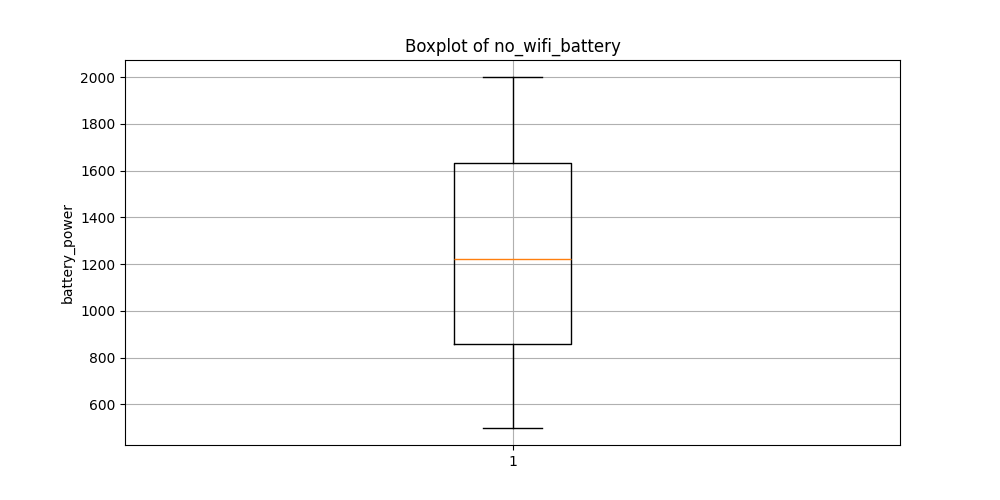
\includegraphics[scale=0.55]{no_wifi_battery_box.png}
        \captionsetup{skip=0pt}
        \caption{Ящик с усами для выборки моделей без Wi-Fi}
        \label{fig:nowifibbox}
    \end{figure}


    \newpage
    Исходя из результирующих графиков можно сделать вывод, что мы верно посчитали характеристики,
    представленные в листинге \ref{mvalsout}.
    На рис. \ref{fig:allbedf} вероятность всегда неубывает, медиана прослеживается
    в районе значения, посчитанного ранее. На рис. \ref{fig:allbhist} столбцы примерно одинаковой высоты --
    распределение скорее всего равномерное. На рис. \ref{fig:allbbox} медиана отмечена
    оранжвой прямой, находится примерно в центре ящика -- распределение данных относительно
    симметрично, и, ее значение совпадает с вычисленным. Интервал между минимумом и максимумом значений в ящике получился
    широким, что подтверждает большое значение вычисленной ранее дисперсии. Выбросы отсутствуют (нет точек вне усов).
    Рассуждения аналогичны для графиков с другой выборкой.
\end{document}